

\chapter{Experiments and Results}
To analyze the adaptability of the SCOUt control schema, three instances of a SCOUtController are trained and then tested and tested in two experiments.
The first experiment compares the performance of each SCOUtController against a random and heuristic controller to observe if they can in fact exhibit intelligent behavior when attempting to complete a goal.
The second experiment tests the adaptability of the controllers' performances when sensors it was trained with are removed, or the goal of the agent is changed.
Two different goals are used in these experiments: Find Human and Map Water.
Find Human requires the agent to search an environment to find a Human anomaly.
Goal completion is either 100 percent for successfully locating the Human, or 0 percent for failing to find the human before depleting health or energy.
For the goal to be successfully completed, the controller must be in one of the eight adjacent cells to the Human anomaly's location in the environment. \todo{photo of human discovery zone}
Map Water tests the controller's ability to navigate an environment and collect as much data for water depth as possible.
Map Water operations will run until the entire area has been mapped, or the agent has depleted its health or energy.
Goal completion is then reward based on the percentage of the environment that was mapped for Water presence.
Training and testing are both conducted using three different EnvironmentTemplates.
Each template differs in difficulty to navigate due to the modifications present within them.

During both training and experimentation, tests are conducted to observe the performance of the controllers.
Each test will compare the intelligent SCOUtController(s) against both random and heuristic controllers.
Two heuristic controllers are used for testing with each goal.
$Heuristic_{FH}$ and $Heuristic_{MW}$ are used for Find Human and Map Water respectively.
The random and heuristic controllers will provide a base line for performance metrics.
This base line is important as the procedural generation of environments could yield conditions that vary the difficulty of achieving the goal, or even prevent goal completion entirely.
When tested against each other, all controllers are given the exact same starting conditions.
Their performances will be compared for the same goal, Environment instance and starting position.
Performance is measured in four categories: goal completion, the number of actions taken, remaining health and remaining energy.
Additionally, the starting location of the controllers for each test will be chosen in a location that does not result in damage (ex: starting in a cell with water present) or immediate goal completion (ex: starting right next to the Human).
The following sections cover the agent setup, environments used and the setup of each test and their results.


\section{Agent}
Similar Agent setup is used for every operation run in training and testing.
The only variation is in the controller being used and the sensor types present.
All health, energy, mobility and durability variables will be set to the same value throughout.
This will assure that no advantage or disadvantage is given to any controller when navigating the environment.
The performance of each controller will then be based solely on the control schema's usage of available sensors and collected environment data.
When sensors are available for an agent's use, the same instance of the sensor type is used.
The exception to this being that the indicator flag for each sensor will differ for the two goals.
For Find Human Temperature and Decibel sensors will be flagged true, and for Map Water the Water sensor will be flagged true.
Each Agent will always begin an Operation with an empty internalMap, 100.0 health and 100.0 energyLevel.
The Agent Mobility and Durabilities and each sensor instance used in experimentation are defined below.

\begin{lstlisting}[language=Scala]
 val mobility = new Mobility(
  movementSlopeUpperThreshHold: 1.0
  movementSlopeLowerThreshHold: -1.0
  movementDamageResistance: 0.0
  movementCost: 0.5
  slopeCost: 0.2
 )
\end{lstlisting}

\begin{lstlisting}[language=Scala]
 val durabilities = List(
  new Duribility (
    elementType: "Water Depth"
    damageUpperThreshold: 0.25
    damageLowerThreshold: infinity
    damageResistance: 0.0
  ),
  new Duribility (
    elementType: "Temperature"
    damageUpperThreshold: 150.0
    damageLowerThreshold: -50.0
    damageResistance: 0.0
  )
 )
\end{lstlisting}

\begin{lstlisting}[language=Scala]
 val elevationSensor = new Sensor (
   elementType: "Elevation"
   range: 30.0
   energyExpense: 0.5
   hazard: true
   indicator: Boolean
 )
\end{lstlisting}

\begin{lstlisting}[language=Scala]
 val waterSensor = new Sensor (
   elementType: "Water Depth"
   range: 1.0
   energyExpense: 1.0
   hazard: true
   indicator: Boolean
 )
\end{lstlisting}

\begin{lstlisting}[language=Scala]
 val temperatureSensor = new Sensor (
   elementType: "Temperature"
   range: 60.0
   energyExpense: 1.0
   hazard: true
   indicator: Boolean
 )
\end{lstlisting}

\begin{lstlisting}[language=Scala]
 val decibelSensor = new Sensor (
   elementType: "Decibel"
   range: 15.0
   energyExpense: 0.1
   hazard: false
   indicator: Boolean
 )
\end{lstlisting}


\section{Environment Templates}
Three EnvironmentTemplates with increasing difficulty are created for use in training and experimentation (EASY, MEDIUM, and HARD).
Increase in difficulty is achieved by increasing the environment size, adding more TerrainModifications, adjusting the average and deviation values for each ElementSeed and reducing the Effects of any Anomalies.
Increased environment size creates a wider area that an Agent will have to search or map to achieve its goal.
More TerrainModifications makes each environment potentially more hazardous.
Changing the average and deviation values of ElementSeeds used to generate the environment has a couple of effects.
First, as an example, by increasing the average decibel values in the environment, the distinction of the Human's decibel effect is dampened and the agent will need to be closer to detect the noise produced.
Also, if the variance in decibel values increases, it becomes more difficult for an agent to distinguish what consuetudes as a significant increase that may indicate the presence of the Human.
Last, by reducing the decibel effect of a Human anomaly itself, the radiation of the effect will cover less area in the environment, meaning the agent will have to search longer before it may pick up on the effect.

Each environment template has one Human that will be placed into it at random in a non-hazardous zone (so not in water).
The same templates will then be used for both the Find Human and Map Water goals.
In the case that the goal is Map Water, a Human anomaly will still be present within the environment, but it will be ignored by the agents.
Each of these EnvironmentTemplates are listed here (\todo{environment templates}) in their Json formats.
This Json format is what appears in each template's respective file.
When a template is used in training and experimentation, it will be loaded in from its file, converted to a Scala object and passed to the EnvironmentBuilder.


\section{Training}
Three separate SCOUtControllers are trained to accumulated memory pools of SAPs.
Once the training phase has completed, these controllers will be tested using their respective memory pools.
During testing, no further SAPs will be added to the controllers' memory pools.
In doing so, a consistent measure of performance can be calculated based on the memory collected during the set training phase defined here.
Each of the three controllers are trained with different goal configurations.
One is trained using the Find Human goal, the second using the Map Water goal and the third is a hybrid, trained using both goals.
They are named $SCOUt_{FH}$, $SCOUt_{MW}$ and $SCOUt_{H}$ respectively.

Each is trained for 30 iterations where an iteration runs one operation per environment template.
Once training has completed, each controller will have collected SAPs from a total of 90 operations (30 on EASY, 30 on MEDIUM and 30 on HARD).
Every operation that $SCOUt_{FH}$ is run in will be with the Find Human goal and every operation for $SCOUt_{MW}$ will be with the Map Water goal.
$SCOUt_{H}$ will alternate goals for each iterations.
In total it will have run 45 operations with the Find Human goal and 45 operations with the Map Water goal (15 on EASY, 15 on MEDIUM and 15 on HARD for both goals).

After each training iteration, the controller is tested with its current memory to track performance improvements.
Testing at each iteration runs a series of simulated operations to collect performance data.
Each series uses the controller's respective goal(s) and is run on each testing environment template 20 times (20 on EASY, 20 on MEDIUM, and 20 on HARD).
The controller tested will have access to its current memory pool that has been gathered in its training so far.
No SAPs will be gathered during these iteration tests.
For a base line, the $Random$ controller is run through the same series of tests.
Results from the 60 total iteration tests will be averaged in each of the four performance categories.
The averaged results of the learning, SCOUt controller will then be differenced against the averaged results of the $Random$ controller.
By differencing the averages, we are observing how much better or worse the SCOUt controller was able to perform than the $Random$ controller in the same testing situation.
This also removes the discrepancy between iteration tests that may have generated a series of exceptionally difficult or easy environments to work within.
It is expected that over training iterations, the goal completion, remaining health and remaining energy will increase, and the number of actions performed will decrease  in comparison to the $Random$ controller.

% The results of each SCOUt controller's training performances over time are found in \todo{training performance}.

Results for $SCOUt_{FH}$ training (figure ~\ref{fig:findhuman_training_results}) show the desired trends of increased performance over training iterations.
Average goal completion and average remaining energy begin at the same performance levels as $Random$ and increase to be consistently better than random over training.
The average number of actions performed begins slightly below $Random$ and continue to decrease before leveling out roughly two-thirds of the way through training.
This demonstrates that the controller is learning to perform more efficiently over time as both average goal completion and average remaining health show major performance boosts while fewer actions are being used.
The average remaining health of $SCOUt_{FH}$ shows slight increase over training, but for the most part is equivalent to that of the $Random$ controller.

\begin{figure}[h]
  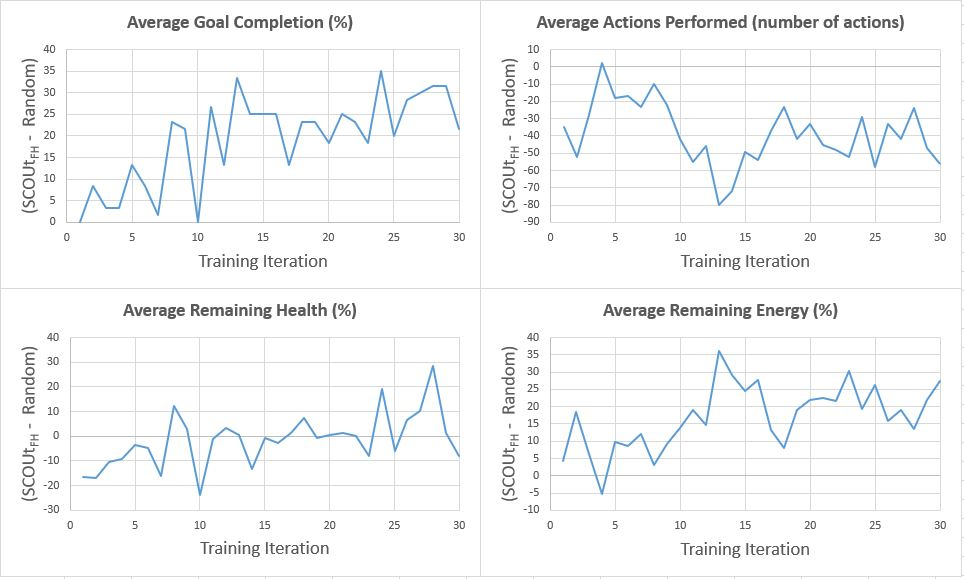
\includegraphics[width=1.0\columnwidth]{Figures/Results/Training/SCOUt-FindHuman.JPG}
  \caption{Training performance results for $SCOUt_{FH}$}
  \label{fig:findhuman_training_results}
\end{figure}

Results for $SCOUt_{MW}$ (figure ~\ref{fig:mapwater_training_results} are less impressive.
Average goal completion and average remaining health both decrease over training, but show upward trends toward the end.
Average remaining health actually performs worse $Random$ throughout iteration testing.
$SCOUt_{MS}$ does perform well in the average number of actions taken per operation, however this is likely due to the fact that health is depleted (agent navigating into water) and the operation is ended early.
The same can be said for the remaining energy, as there will be a large amount of energy remaining after an operation is ended due to depletion of health.
The reason for these poor performance results seem to be tied with the agents inability to avoid hazardous water areas.
It is believed that the long term reward equation \todo{ref eq} did not provide adequate values for the controller to learn from because of the goal completion reward for Map Water in combination with the available energy for the agent to use.
Map Water goal completion is measured by the percent of the environment that has successfully been scanned for water.
In ~\ref{sec:experiment1}, we will see that all controllers have an average goal completion rate below 40 percent on EASY environments, below 30 percent on MEDIUM, and below 15 percent on HARD.
Poor goal completion scores will result in poor long term rewards.
The reinforcement learning schema will have difficulty making clear distinctions between "good" and "bad" actions when all SAPs in the memory pool contain low long term rewards.

\begin{figure}[h]
  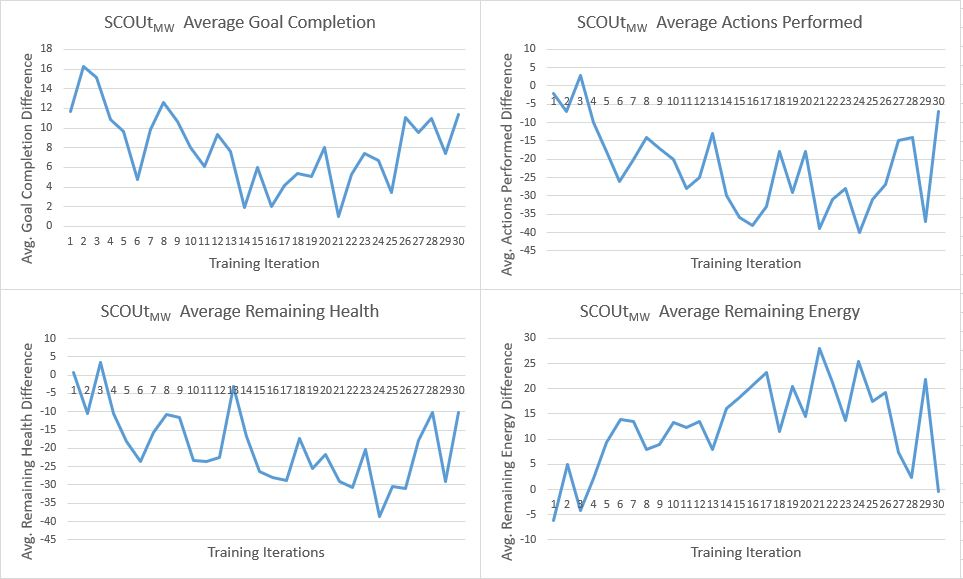
\includegraphics[width=1.0\columnwidth]{Figures/Results/Training/SCOUt-MapWater.JPG}
  \caption{Training performance results for $SCOUt_{MW}$}
  \label{fig:mapwater_training_results}
\end{figure}

$SCOUt_{H}$ does not show any change in performance throughout training.
This can likely be attributed to the cancelation of good performance on Find Human mixed with poor performance on Map Water.
Iteration testing is done with both goals and results from operations with both goal types are averaged together.
Outside of average remaining health, the hybrid controller does consistently perform better than $Random$.
Performance levels are still not as high as seen in $SCOUt_{FH}$, likely due to the same issue discussed in $SCOUt_{MW}$'s results, where poor long term rewards are diluting the controller's memory pool.

\begin{figure}[h]
  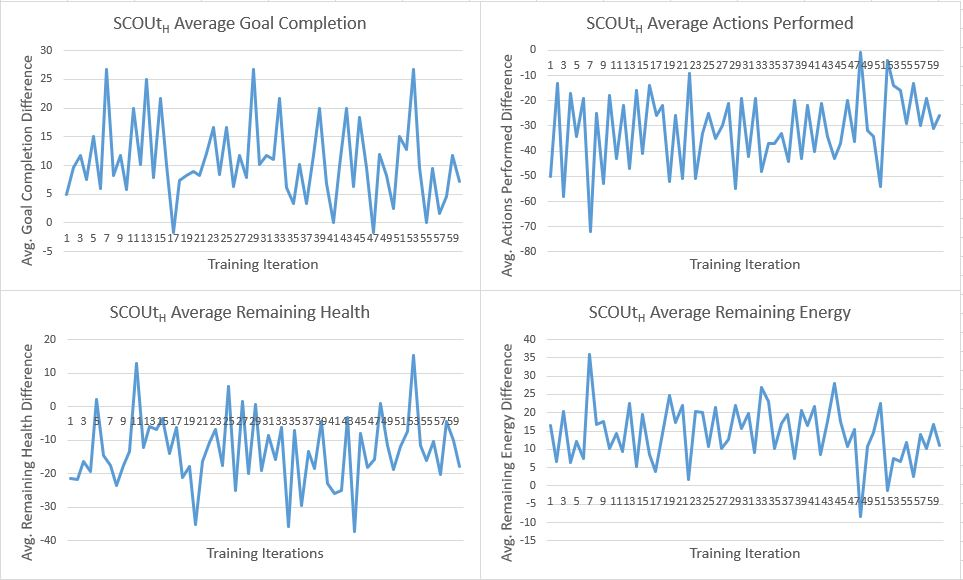
\includegraphics[width=1.0\columnwidth]{Figures/Results/Training/SCOUt-Hybrid.JPG}
  \caption{Training performance results for $SCOUt_{H}$}
  \label{fig:hybrid_training_results}
\end{figure}



\section{Experiment 1} \label{sec:experiment1}
Once training has completed, the resulting SCOUt controllers are individually tested against $Random$ and respective heuristic controllers.
Test in Experiment 1 run a total of 1000 operations per environment template.
The environment template is used to generate 200 unique environments, each of which is used in 5 operations.
Performance results are averaged for each controller and compared under the three test environment templates.

\todo{Find Human}

\begin{figure}[h]
  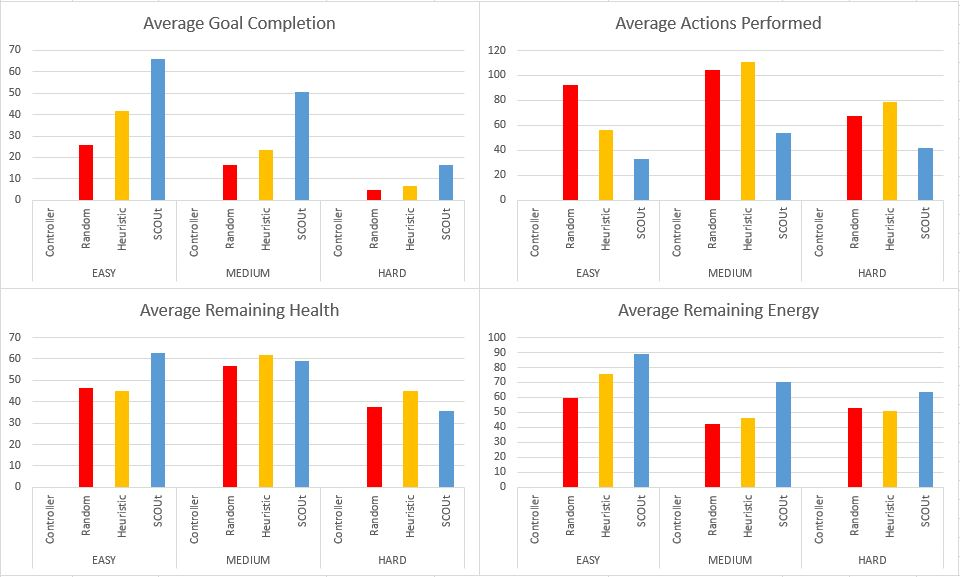
\includegraphics[width=1.0\columnwidth]{Figures/Results/Experiment1/FindHuman.JPG}
  \caption{Performance results for $Random$, $Heuristic_{FH}$ and $SCOUt_{FH}$ on Find Human goal in different environment difficulties.}
  \label{fig:findhuman_test_results}
\end{figure}


\todo{Map Water}

\begin{figure}[h]
  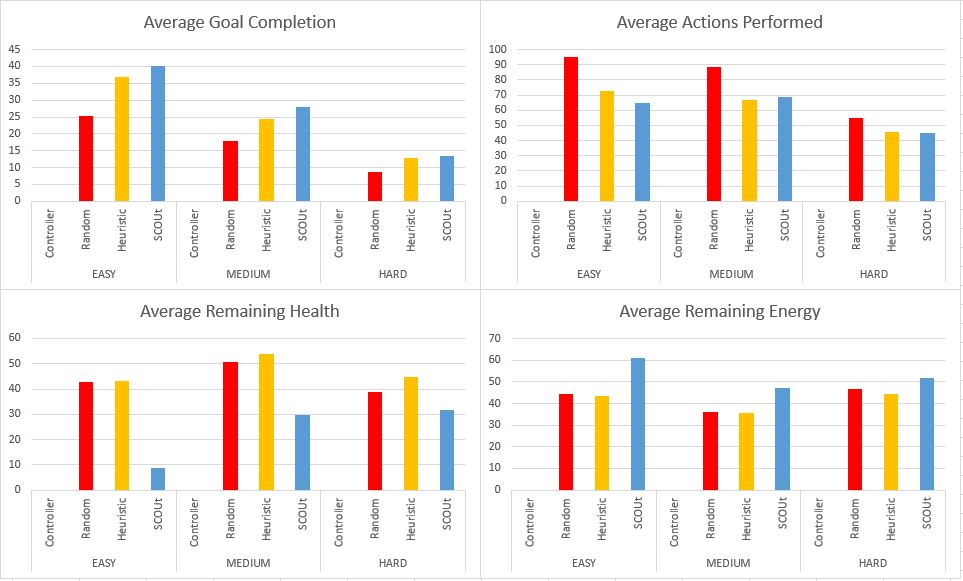
\includegraphics[width=1.0\columnwidth]{Figures/Results/Experiment1/MapWater.JPG}
  \caption{Performance results for $Random$, $Heuristic_{MW}$ and $SCOUt_{MW}$ on Map Water goal in different environment difficulties.}
  \label{fig:mapwater_test_results}
\end{figure}


\todo{Hybrid}

\begin{figure}[h]
  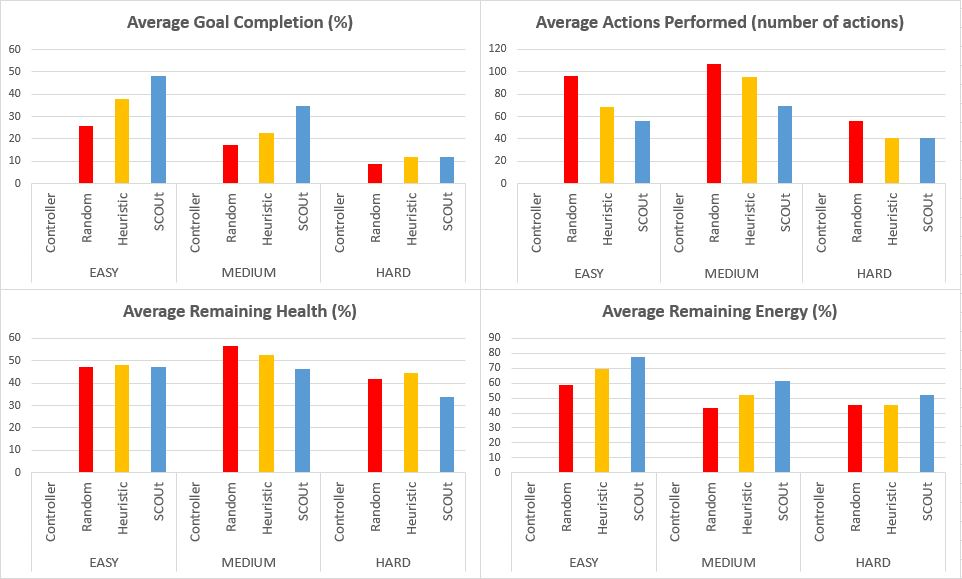
\includegraphics[width=1.0\columnwidth]{Figures/Results/Experiment1/HybridFindHuman.JPG}
  \caption{Performance results for $Random$, $Heuristic_{FH}$ and $SCOUt_{H}$ on Find Human goal in different environment difficulties.}
  \label{fig:hybrid_findhuman_test_results}
\end{figure}

\begin{figure}[h]
  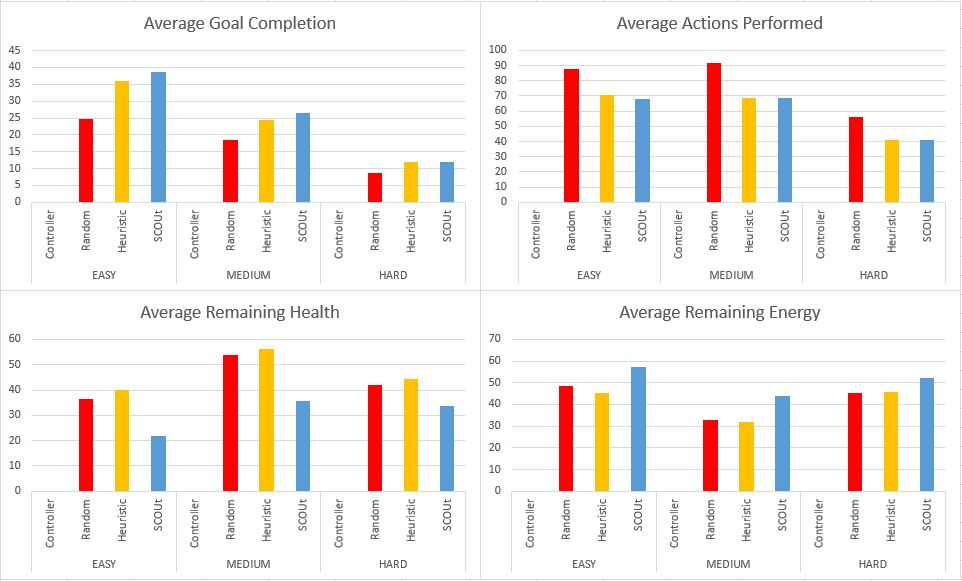
\includegraphics[width=1.0\columnwidth]{Figures/Results/Experiment1/HybridMapWater.JPG}
  \caption{Performance results for $Random$, $Heuristic_{MW}$ and $SCOUt_{H}$ on Map Water goal in different environment difficulties.}
  \label{fig:hybrid_mapwater_test_results}
\end{figure}





\section{Experiment 2} \label{sec:experiment2}
The second experiment is broken into three tests: goal changing, sensor set changing and additional training.

Goal changing tests the performance of $SCOUt_{FH}$ on the Map Water goal and the performance of $SCOUt_{MW}$ on the Find Human goal.
The SCOUt controllers will have no training on the new goal they are tested within.
This will exhibit their ability to complete a goal using only memory from the original goal they were trained on.
